\section{NP-complete problems involving sets and numbers.}

\subsection{Disposition}

\begin{enumerate}
 \item \textbf{Def. P, NP, NP-hard \& NPC}
    \subitem  Tegn!
 \item \textbf{Def. Reduktioner}
    \subitem  Proposition 3: Transitivitet (v. bevis)
    \subitem  Proposition 4: Nedadgående lukkethed af P  
 \item \textbf{Lemma 7:} \textit{Hvis $L_1 \in$ NP-hard og $L_1 \leq L_2$, så er $L_2 \in$ NP-hard}
    \subitem  Bevis. (måske)
 \item \textbf{Reduktionstræ}
 \item \textbf{Proposition 9.2:} \textit{3SAT $\in$ NPC}
    \subitem Vis SAT $\leq$ 3SAT. (måske)
 \item \textbf{Theorem 9.9:} \textit{3SAT $\leq$ TRIPARTITE MATCHING}
    \subitem Bevis
 \item \textbf{Collary:} \textit{EXACT COVER BY 3-SETS, SET COVERING and SET PACKING are NPC}
    \subitem Vis for EXACT COVER BY 3-SETS
 \item \textbf{Theorem:} \textit{EXACT COVER BY 3-SETS $\leq$ KNAPSACK}
    \subitem Bevis
\end{enumerate}

\subsection{Emne detaljer}

Følgende afsnit indeholder detaljer om hvert punkt i dispositionen ovenfor (og muligvis flere ting også).

\subsubsection{Def. P, NP, NP-hard \& NPC}

Lad os starte med lige at kigge på de kompleksitetsklasser vi har arbejdet med her i kurset.
\begin{center}
 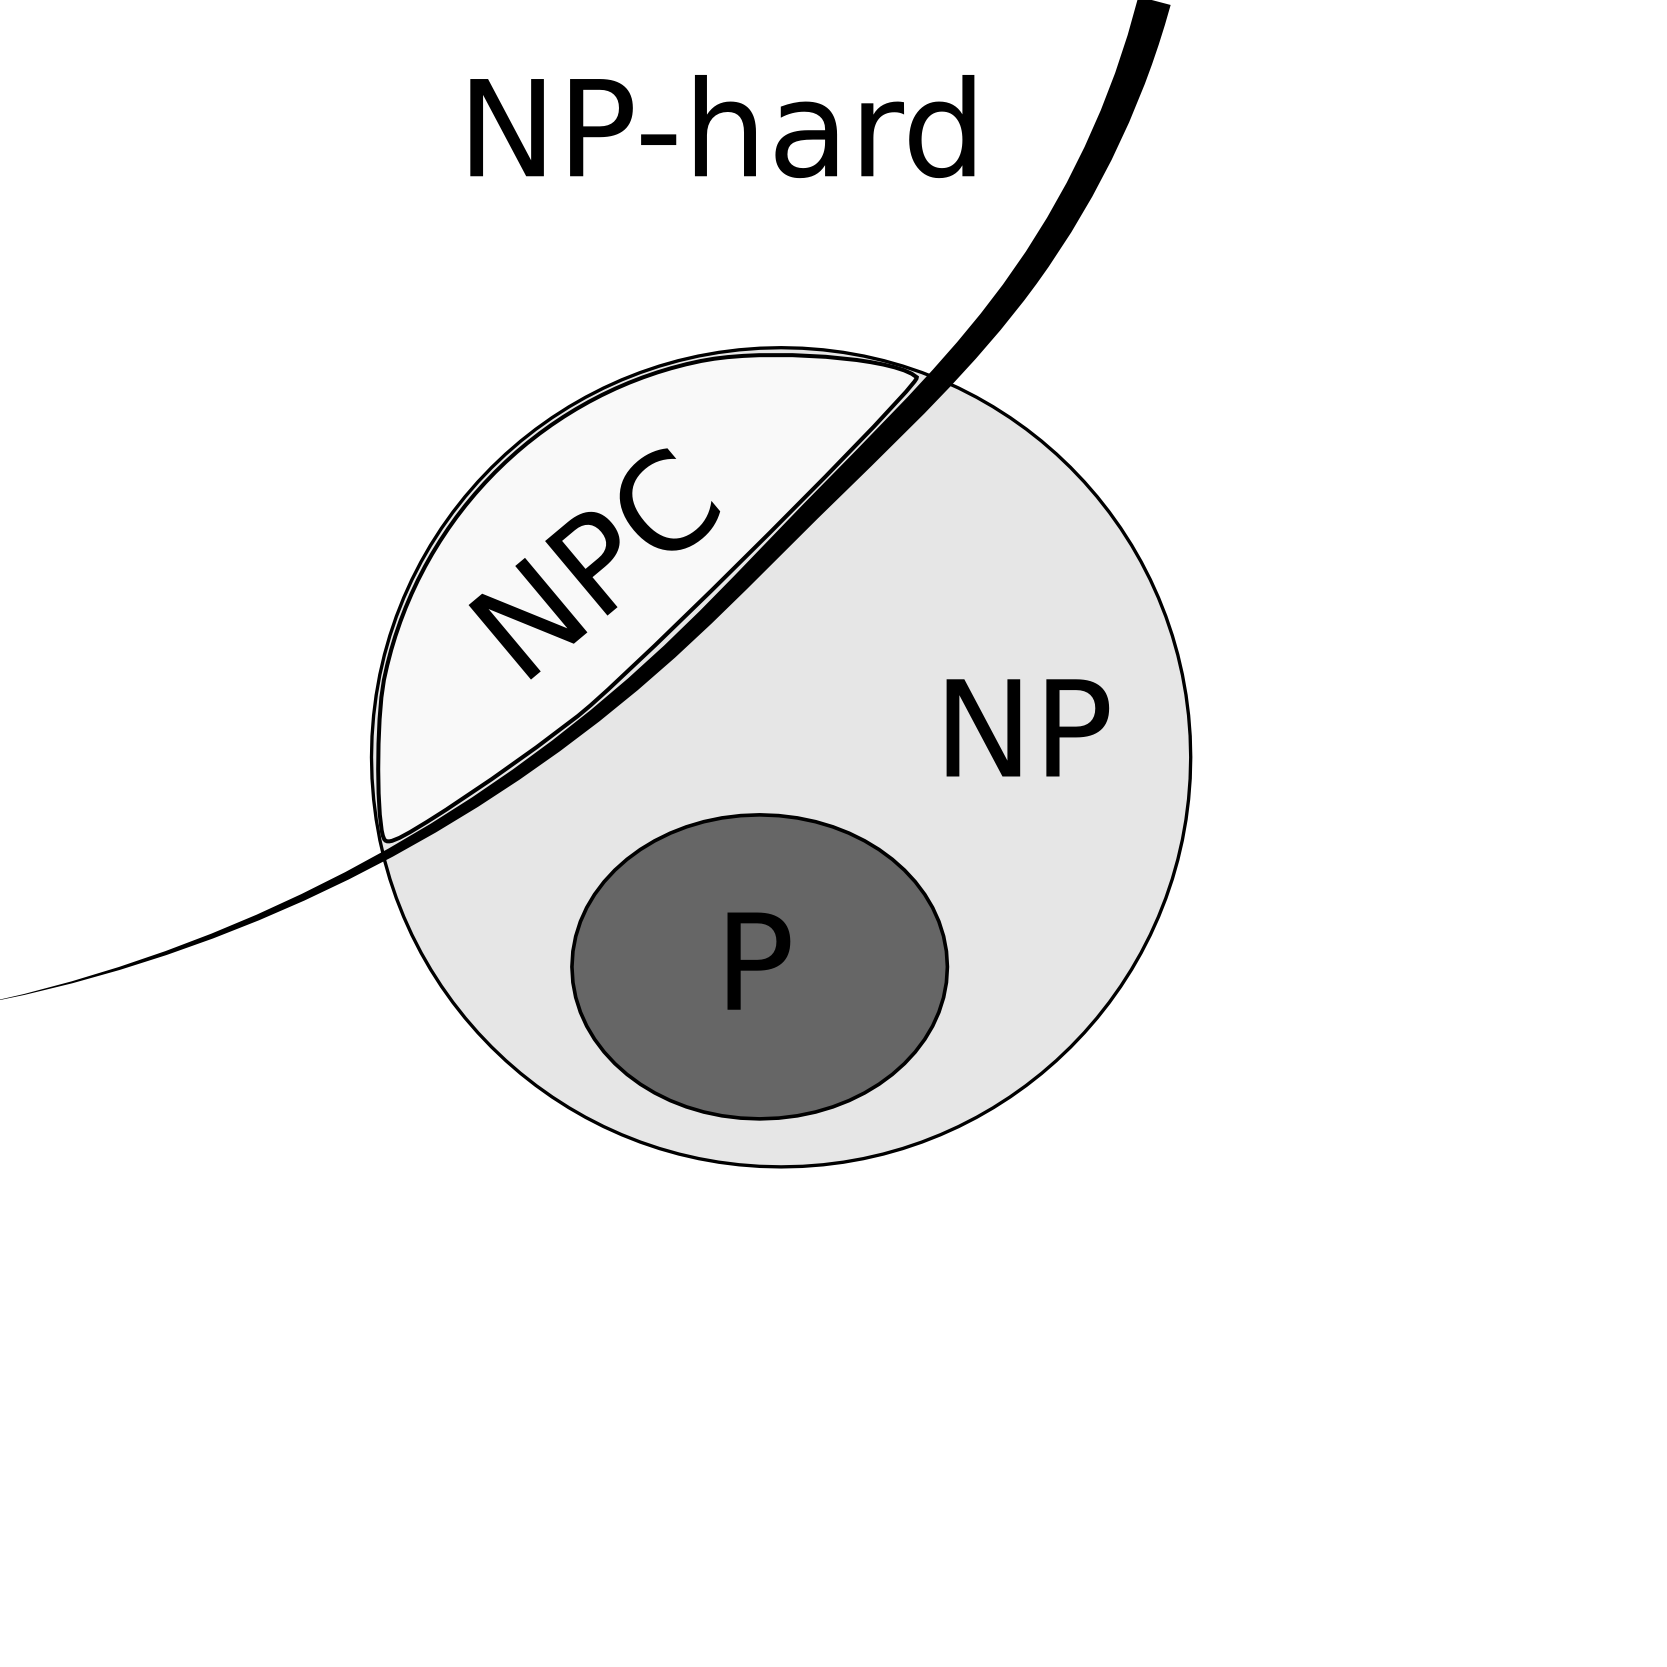
\includegraphics[bb=0 0 400 400,scale=0.3]{./PNPNPC.png}
 % PNPNPC.png: 1667x1667 pixel, 300dpi, 14.11x14.11 cm, bb=0 0 400 400
\end{center}


\paragraph{P}
~\\
~\\
Kompleksitetsklassen $P$ er formelt defineret således:
\begin{align*}
 P = \left\lbrace L \subseteq \left\lbrace 0,1 \right\rbrace^* | \exists \text{ TM } M_L \text{ der afgører L i polynomiel tid } \right\rbrace
\end{align*}
Altså klassen af beslutningsproblemer der kan blive bestemt af en deterministisk Turing Maskine hvor antallet af ``steps'' maskinen udfører for et givent $x$ maksimalt er $\rho(x)$ for et givent polynomiel $\rho$.\\
 
Intuivit ser vi kompleksitetsklassen $P$ som en klasse for problemer for hvilket vi kender en effektiv løsning. Altså ethvert problem med worst-case kørselstid på formen $O(n^k)$ for et givent $k$.

At worst-case kørseltid på et problem er polynomiel betyder dog ikke reelt at det er et nemt problem (modsat hvad Cobham's Thesis påstår). I hele den analyse ignorerer vi fuldkommen konstanter, samt forventet kørselstid som I mange tilfælde kan få ``sværere'' problemer til at køre bedre end ``nemme'' problemer i $P$.


\paragraph{NP}
~\\
~\\
Kompleksitetsklassen $NP$ er lidt mere kluntet formelt defineret, så vi starter lige med intuitionen først.

Intuitivt kan $NP$ ses som klassen af beslutningsproblemer for hvilket ``yes'' instanserne kan verificeres i polynomiel tid på en deterministisk Turing Maskine. Altså er det komplekse problemer med eksponentiel løbetid, men hvor løsningen til et sådant problem nemt kan verificeres til at være korrekt.\\
~\\
Kompleksitetsklassen $NP$ er formelt defineret således:
\begin{align*}
 NP = \left\lbrace L \subseteq \left\lbrace 0,1 \right\rbrace^* | \exists \rho \in Z[x], L' \in P, \forall x \in \left\lbrace 0,1 \right\rbrace^* : ( x \in L \Leftrightarrow \exists y \in \left\lbrace 0,1 \right\rbrace^* : |y| \leq \rho(|x|) \wedge \left\langle x,y \right\rangle \in L') \right\rbrace
\end{align*}
Definitionen skal forståes således: Vi har et sprog $L' \in P$, samt et polynomiel $\rho$. Vi tænker så nu på et sæt af binære strenge af længde maksimalt $\rho(|x|)$, hvor disse representerer mulige løsninger til probleminstansen $x$. Med denne fortolkning bliver $\left\langle x,y \right\rangle \in L'$ så måden hvorpå vi tester om en given løsning $y$ virkelig er en korrekt løsning. 

Denne form for søgningsproblem kaldes ofte for et simpelt søgningsproblem, da den kan verificeres i polynomiel tid, men ikke løses deri (antaget $P \neq NP$).\\

For at løse et givent NP problem kunne vi så løbe igennem alle mulige løsninger for $y$, som sammenlagt ville være $2^{\rho(|x|)+1}-1$, og for hver af dem tjekke $\left\langle x,y \right\rangle \in L'$. Det ønsker vi dog ikke, da det ville tage eksponentiel tid. I stedet forsøger man ofte at finde snedige måder at lave speed-ups og/eller lave approximationsalgoritmer af forskellige art.

Og i visse tilfælde er man også heldig at finde en algoritme i $P$ for et $NP$ problem, hvorved man har vist at problemet i virkeligheden ligger i $P$ som jo er et subset af $NP$.

\paragraph{NP-hard}
~\\
~\\
Et sprog defineres som NP-hard såfremt der gælder:

\begin{align*}
 \forall L' \in NP: L' \leq L
\end{align*}

Altså gælder der, at ethvert sprog $L'$ i NP kan reduceres til $L$. Intuitionen er her, at algoritmen til at løse NP-hard problemet er så stærk (eller generel) at den kan bruges til at løse ethvert andet problem i NP. Man siger desuden, at et NP-hard problem således er mindre sandsynlig end noget andet sprog i NP, til at være i P.\\

Navnet kan dog være lidt forvirrende, da et NP-hard problem faktisk ikke behøver være i NP og hvis de er, så kaldes de faktisk ikke engang bare NP-hard længere.

\paragraph{NPC}
~\\
~\\
NP-Complete (NPC) er den særlige klasse af problemer der både er NP-hard og befinder sig i NP. Formelt defineret således: 

\begin{align*}
 NPC = \left\lbrace L \in \left\lbrace 0,1 \right\rbrace^* | L \in NP \wedge (\forall L' \in NP: L' \leq L) \right\rbrace
\end{align*}

NPC problemer er særligt interessante, da vi kan bruge dem til at bevise et givent problem er NP-Complete, således vi ikke spilder tid på forsøg med at finde en algoritme i $P$ for problemet (antaget $P\neq NP$). Dette gør vi vha. noget vi kalder reduktioner.

\subsubsection{Def. Reduktioner}

Det bringer os så til en grundlæggende metode i computationel kompleksitetsteori, nemlig reduktioner. Først og fremmest den formelle definition.

Givet to sprog $L_1$ og $L_2$, en polynomiel reduktion $r$ af $L_1$ til $L_2$ er en polynomial time computable map for hvilken der gælder:

\begin{align*}
 \forall x : x \in L_1 \text{ hviss. } r(x) \in L_2
\end{align*}

Dette skrives som $L_1 \leq L_2$, hvor man læser det som at $L_1$ reduceres til $L_2$. Intuitivt betyder reduktion blot, at vi kan oversætte enhver given instans af $L_1$ til en anden instans af $L_2$. Vi siger desuden, at $L_2$ er et mere generelt sprog end $L_1$ og kan derfor ses, som værende mere sandsynlig til ikke at være i $P$.


Herudover har  reduktioner desuden to nyttige egenskaber vi skal bruge senere.

\paragraph{Proposition 3: Hvis $L_1 \leq L_2$ og $L_2 \leq L_3$, så gælder der $L_1 \leq L_3$}
~\\
~\\
Denne proposition underbygger, at reduktioner er transitive. Vi beviser den således:

\begin{proof}
 Vi har polynomial time computable maps $r_1()$ og $r_2()$, hvor følgende ting gælder:

\begin{itemize}
 \item For ethvert $x$ gælder der, at $x \in L_1$ hvis og kun hvis $r_1(x) \in L_2$.
 \item For ethvert $y$ gælder der, at $y \in L_2$ hvis og kun hvis $r_2(y) \in L_3$.
\end{itemize}

Således har vi for alle $x$, at $x \in L_1$ hvis og kun hvis $r_2(r_1(x)) \in L_3$. Og siden vi blot har brugt to polynomial time computable maps efter hinanden (hvormed det hele kan ses som en polynomial time computable map), så har vi $L_1 \leq L_3$.
\end{proof}

\paragraph{Proposition 4: Hvis $L_1 \leq L_2$ og $L_2 \in P$, så er $L_1 \in P$.}

Proposition 4 siger intuitivt, at $P$ er lukket nedad under reduktion. 


\subsubsection{Cook's Theorem}

Vi vil jo gerne kunne vise at diverse problemer er NP-Complete, men for at gøre det vha. reduktioner, så skal vi først have et NP-Complete problem at starte ud fra.

Takket være Stephen Cook fik vi i 1972 netop lige det, da han viste at SATISFIABILITY PROBLEMET, forkortet SAT, var NP-hard. Herefter kunne mange andre så bruge SAT til at reducere til andre problemer, for at vise at disse nye problemer var NP-hard. Cook beviste oprindeligt SAT ved at vise alle problemer i NP reducerede til SAT, hvilket er en noget kompliceret affære. Derfor har vi i dette kursus i stedet vist et relateret problem CIRCUIT SAT er NP-hard og så reduceret dette til SAT.

Det vil vi dog ikke gøre til dette emne og vil i stedet blot definere problemerne samt deres kompleksitet, så vi kan bruge dem til at lave andre reduktioner.

\begin{itemize}
 \item CIRCUIT SAT $\in$ NPC (Theorem 11)
 \item CIRCUIT SAT $\leq$ SAT (Proposition 12)
\end{itemize}

\paragraph{Def. SAT}
~\\
~\\
Givet en CNF formel, er der en tildeling af sandt/falsk til variablerne således hele udtrykket evaluerer til sandt?\\

\paragraph{Def. CIRCUIT SAT}
~\\
~\\
Givet et boolsk kredsløb $C$, er der en inputvektor $x \in \left\lbrace 0,1 \right\rbrace^n$ således at $C(x) = 1$?

\subsubsection{Proposition 9.2}

Vi ved som sagt, at SAT er et NP-Complete problem, så kan vi bruge det til at bevise andre problemer er NP-Complete ved at reducere SAT til dem.
Specifikt er det planen at gennemgå følgende reduktioner i løbet af dette emne:
\begin{center}
 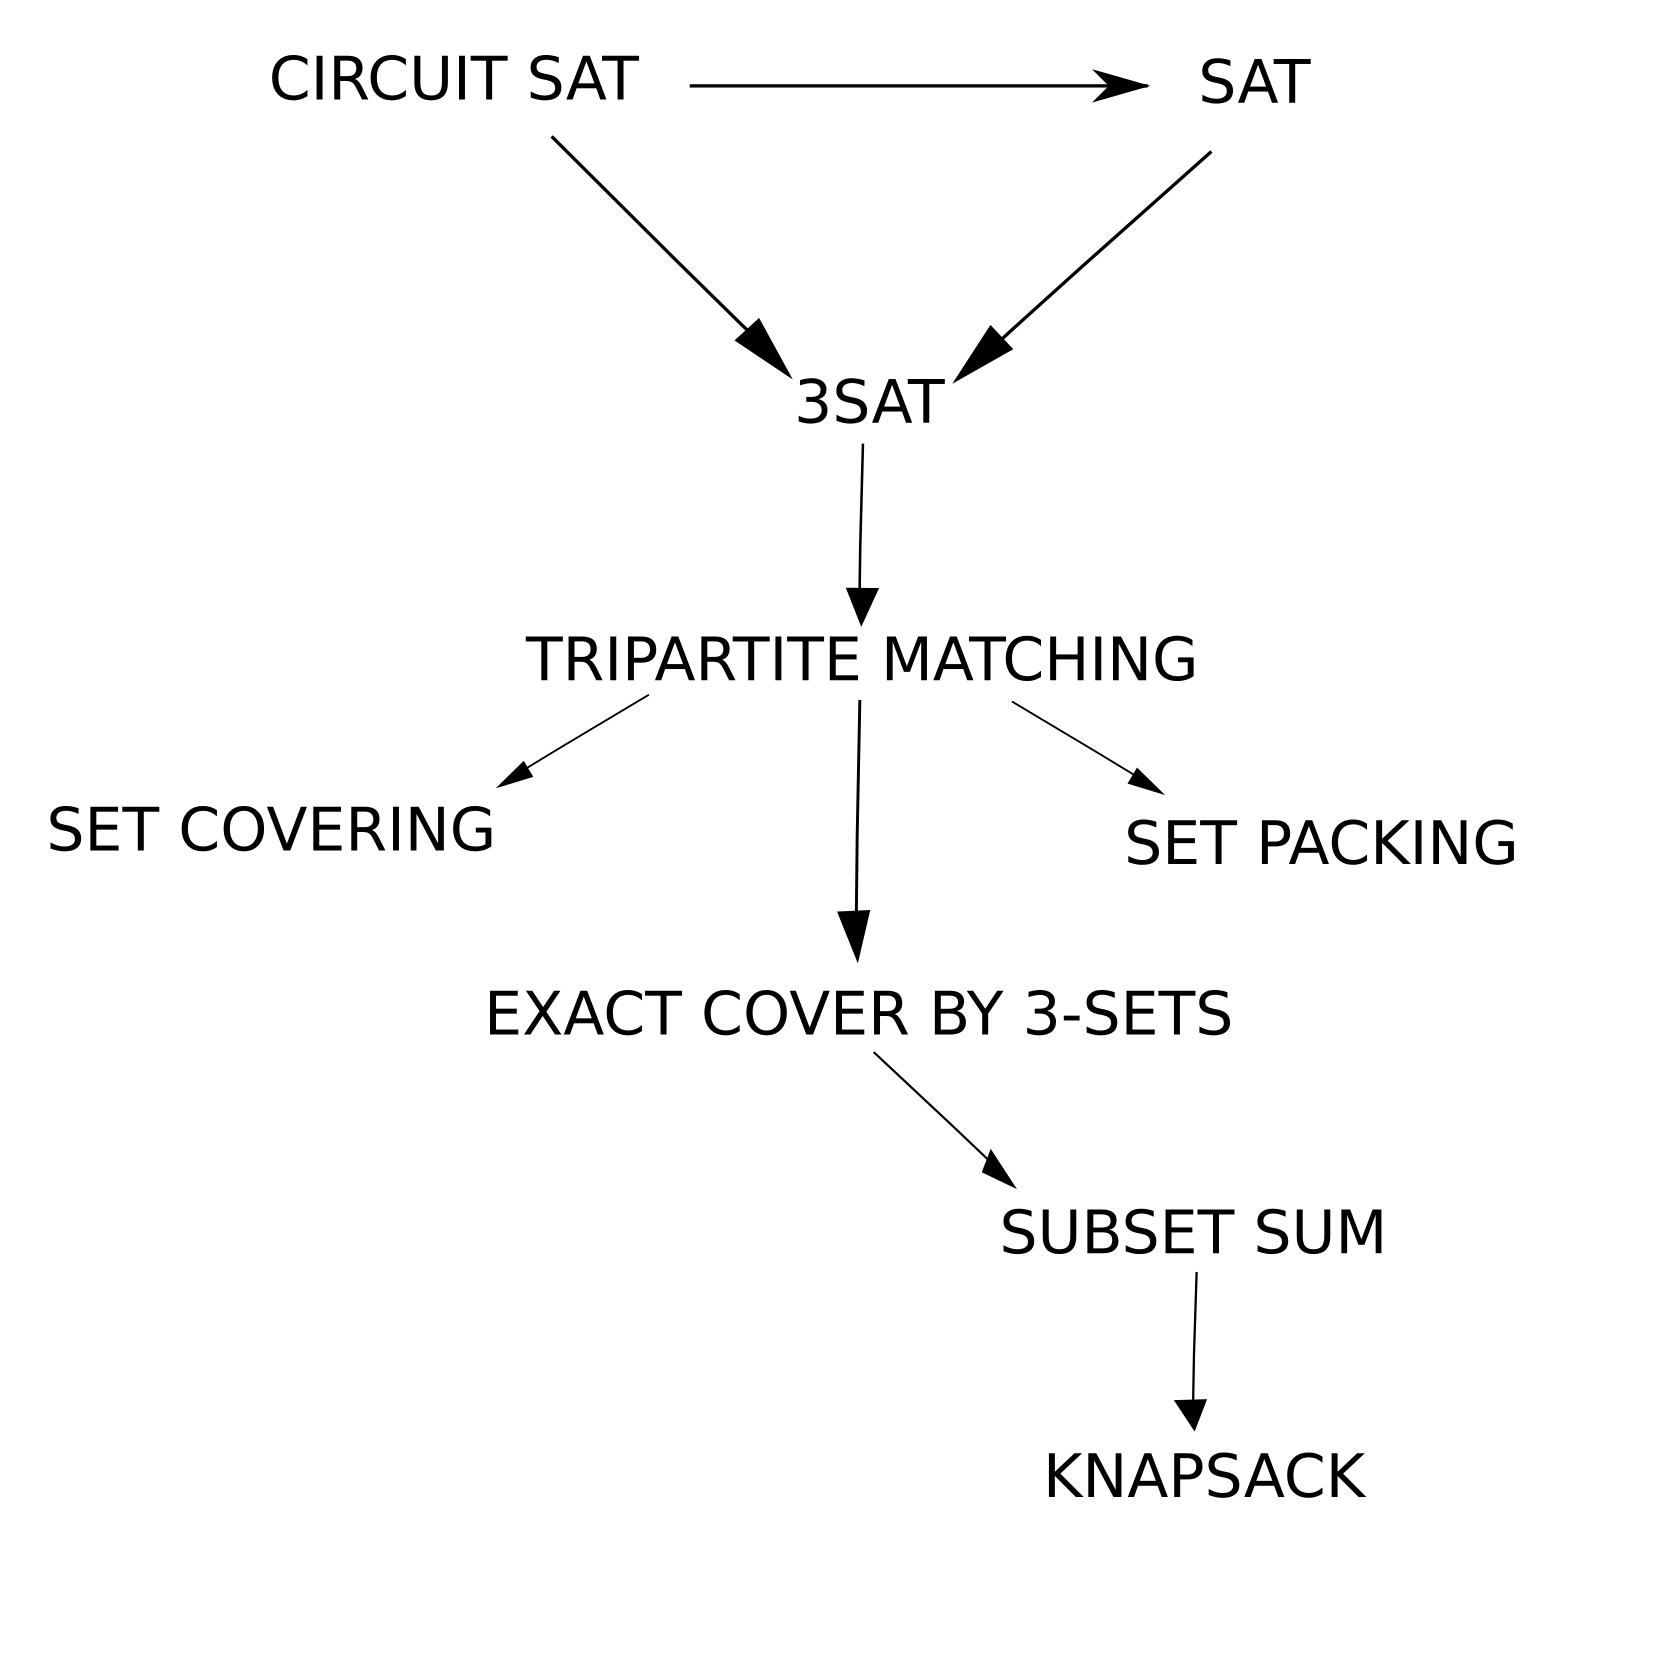
\includegraphics[bb=0 0 400 400,scale=0.5]{./GraphReductionTreeSetNumbers.png}
 % GraphReductionTree.png: 1667x1667 pixel, 300dpi, 14.11x14.11 cm, bb=0 0 400 400
\end{center}

Vi vil derfor tage et simpelt eksempel først ved at reducere til en special case af SAT, kaldet 3SAT.\\
3SAT er en special case af SAT hvor hver klausul skal indeholde præcis 3 literals. Det er et specifikt eksempel på kSAT hvor $k \geq 1$.\\
~\\
\textbf{Proposition 9.2:} 3SAT $\in$ NPC

\begin{proof}
 Vi vil, som sagt, vise at 3SAT $\in$ NPC ved at lave en reduktion fra SAT, således vi bruger et polynomial time computable map til at oversætte enhver instans af SAT til en instans af 3SAT. 

Givet en CNF formel $f$ i SAT vil vi konstrukere en ny CNF formel $f' = r(x)$ i 3SAT med 3 literals i hver klausul. $r$ er således vores polynomial time computable map der ændrer følgende i $f$:\\

For hver klausul $k$ i $f$ med literals $x_1, \hdots, x_{|k|}$ ændres:
\begin{itemize}
 \item Hvis $|k| = 2$: Dupliker klausulen og tilføj en ny variabel i begge hvor den negeres i anden klausul \\
      $(x_1 \vee x_2) \rightarrow (x_1 \vee x_2 \vee u) \wedge (x_1 \vee x_2 \vee \neg u)$
 \item Hvis $|k| = 1$: Gør som ved $|k| = 2$, men gør det to gange \\
      $(x_1) \rightarrow (x_1 \vee u_1) \wedge (x_1 \vee \neg u_1) \rightarrow (x_1 \vee u_1 \vee u_2) \wedge (x_1 \vee u_1 \vee \neg u_2) \wedge (x_1 \vee \neg u_1 \vee u_2) \wedge (x_1 \vee \neg u_1 \vee \neg u_2)$
 \item Hvis $|k| = 3$: Gør vi ingenting
 \item Hvis $|k| > 3$: Da vi har en klausul $(x_1,\hdots,x_{|k|})$ så skal vi have en generel måde hvorpå vi kan konvertere dette til klausuler med 3 literals. Måden vi gør det på er ved at lave nye variabler $u_1,\hdots,u_{|k|-3}$ og lave en ``kaskade'' af disse:\\
      $(x_1,\hdots,x_{|k|}) \rightarrow (x_1 \vee x_2 \vee u_1) \wedge (x_3 \vee \neg u_1 \vee u_2) \wedge \hdots \wedge (x_{k-2} \vee \neg u_{k-4} \vee u_{k-3}) \wedge (x_{k-1} \vee x_k \vee \neg u_{k-3})$ \\
      ~\\
      Længden af denne udvidelse er så $|k|-2$.
      For at se at vi kan gøre dette, så skal vi kigge på hvorledes det gamle udtryk har set ud. Hvis det gamle udtryk har været sandt så har et af $x_i$'erne været sat til true. Hvis vi så sætter alle $u_i$'er til true op til punktet hvor $x_i$ blev mødt og falsk derefter, så kan vi se, at det giver et samlet sandt udtryk som før. Det betyder også at hvis ingen $x_i$'er er sat til true og det samlede udtryk derfor burde være falsk, så har vi også bibeholdt dette i oversættelsen, da alle $u_i$'erne derfor må være false.\\
      ~\\
      \textbf{TODO:} Ovenstående trin for $|k| > 3$ er IKKE rigtig. Jeg har ikke haft tid til at rette det.. Søg på Google og find det rigtige svar. Der findes sider der beskriver beviset.
\end{itemize}

En tilfredsstillende assignment for $f'$ vil altså også være tilfredsstillende for $f$ og vice-versa. Vi har således lavet en reduktion vha. et polynomial time computable map $r$, hvor længden af $f'$ maksimalt er $O(|f|^2)$.

Vi har derfor nu vist, at SAT $\leq$ 3SAT, hvorfor vi kan konkludere at 3SAT $\in$ NPC.
\end{proof}

\subsubsection{Theorem 9.9}

\textbf{TODO: } Følgende bevis har jeg ikke ordentligt forstået og kan meget vel være forkert hernede.. Tjek den efter meget grundigt og få ekstra kilder hvorfra du kan verificere nedenstående.. Beviset fuldføres heller ikke helt, som kan ses nedenfor. \\
~\\
Nu hvor vi har fastlagt at 3SAT er i NPC, så kan vi bruge den til at reducere videre. Så det første vi vil kigge på er et beslutningsproblem relateret til set, kaldet TRIPARTITE MATCHING (oversat: treparts matching)

TRIPARTITE MATCHING problemet er følgende: Vi er givet tre sæt $B$, $G$ og $H$ respektivt indeholdende drenge, piger og hjem. Hvor hver af disse sæt indeholder $n$ elementer og vi har en relation $T \subseteq B \times G \times H$. Findes der nu et sæt af $n$ tripler i $T$, hvor ingen to af disse har komponenter til fælles. \\

Altså sagt på en anden måde, kan vi finde $n$ tripler hvor hver dreng er koblet med en pige og disse så er placeret i et hjem.

Dette problem er NP-Complete, hvilket vi så nu vil vise.
\\
~\\
\textbf{Theorem 9.9:} TRIPARTITE MATCHING $\in$ NPC

\begin{proof}
 Vi vil vise at TRIPARTITE MATCHING er i NPC ved at reducerer fra 3SAT. Vi har altså en CNF formel $f$ i 3SAT med variabler $x_1,\hdots,x_n$ og skal så nu konstruere instanser af TRIPARTITE MATCHING på baggrund af dette vha. en polynomieltids reduktion $r$.

 Måden hvorpå vi konstruerer disse instanser er vha. en såkaldt ``choice-consistency'' gadget, som illustreret nedenfor.
 \begin{center}
 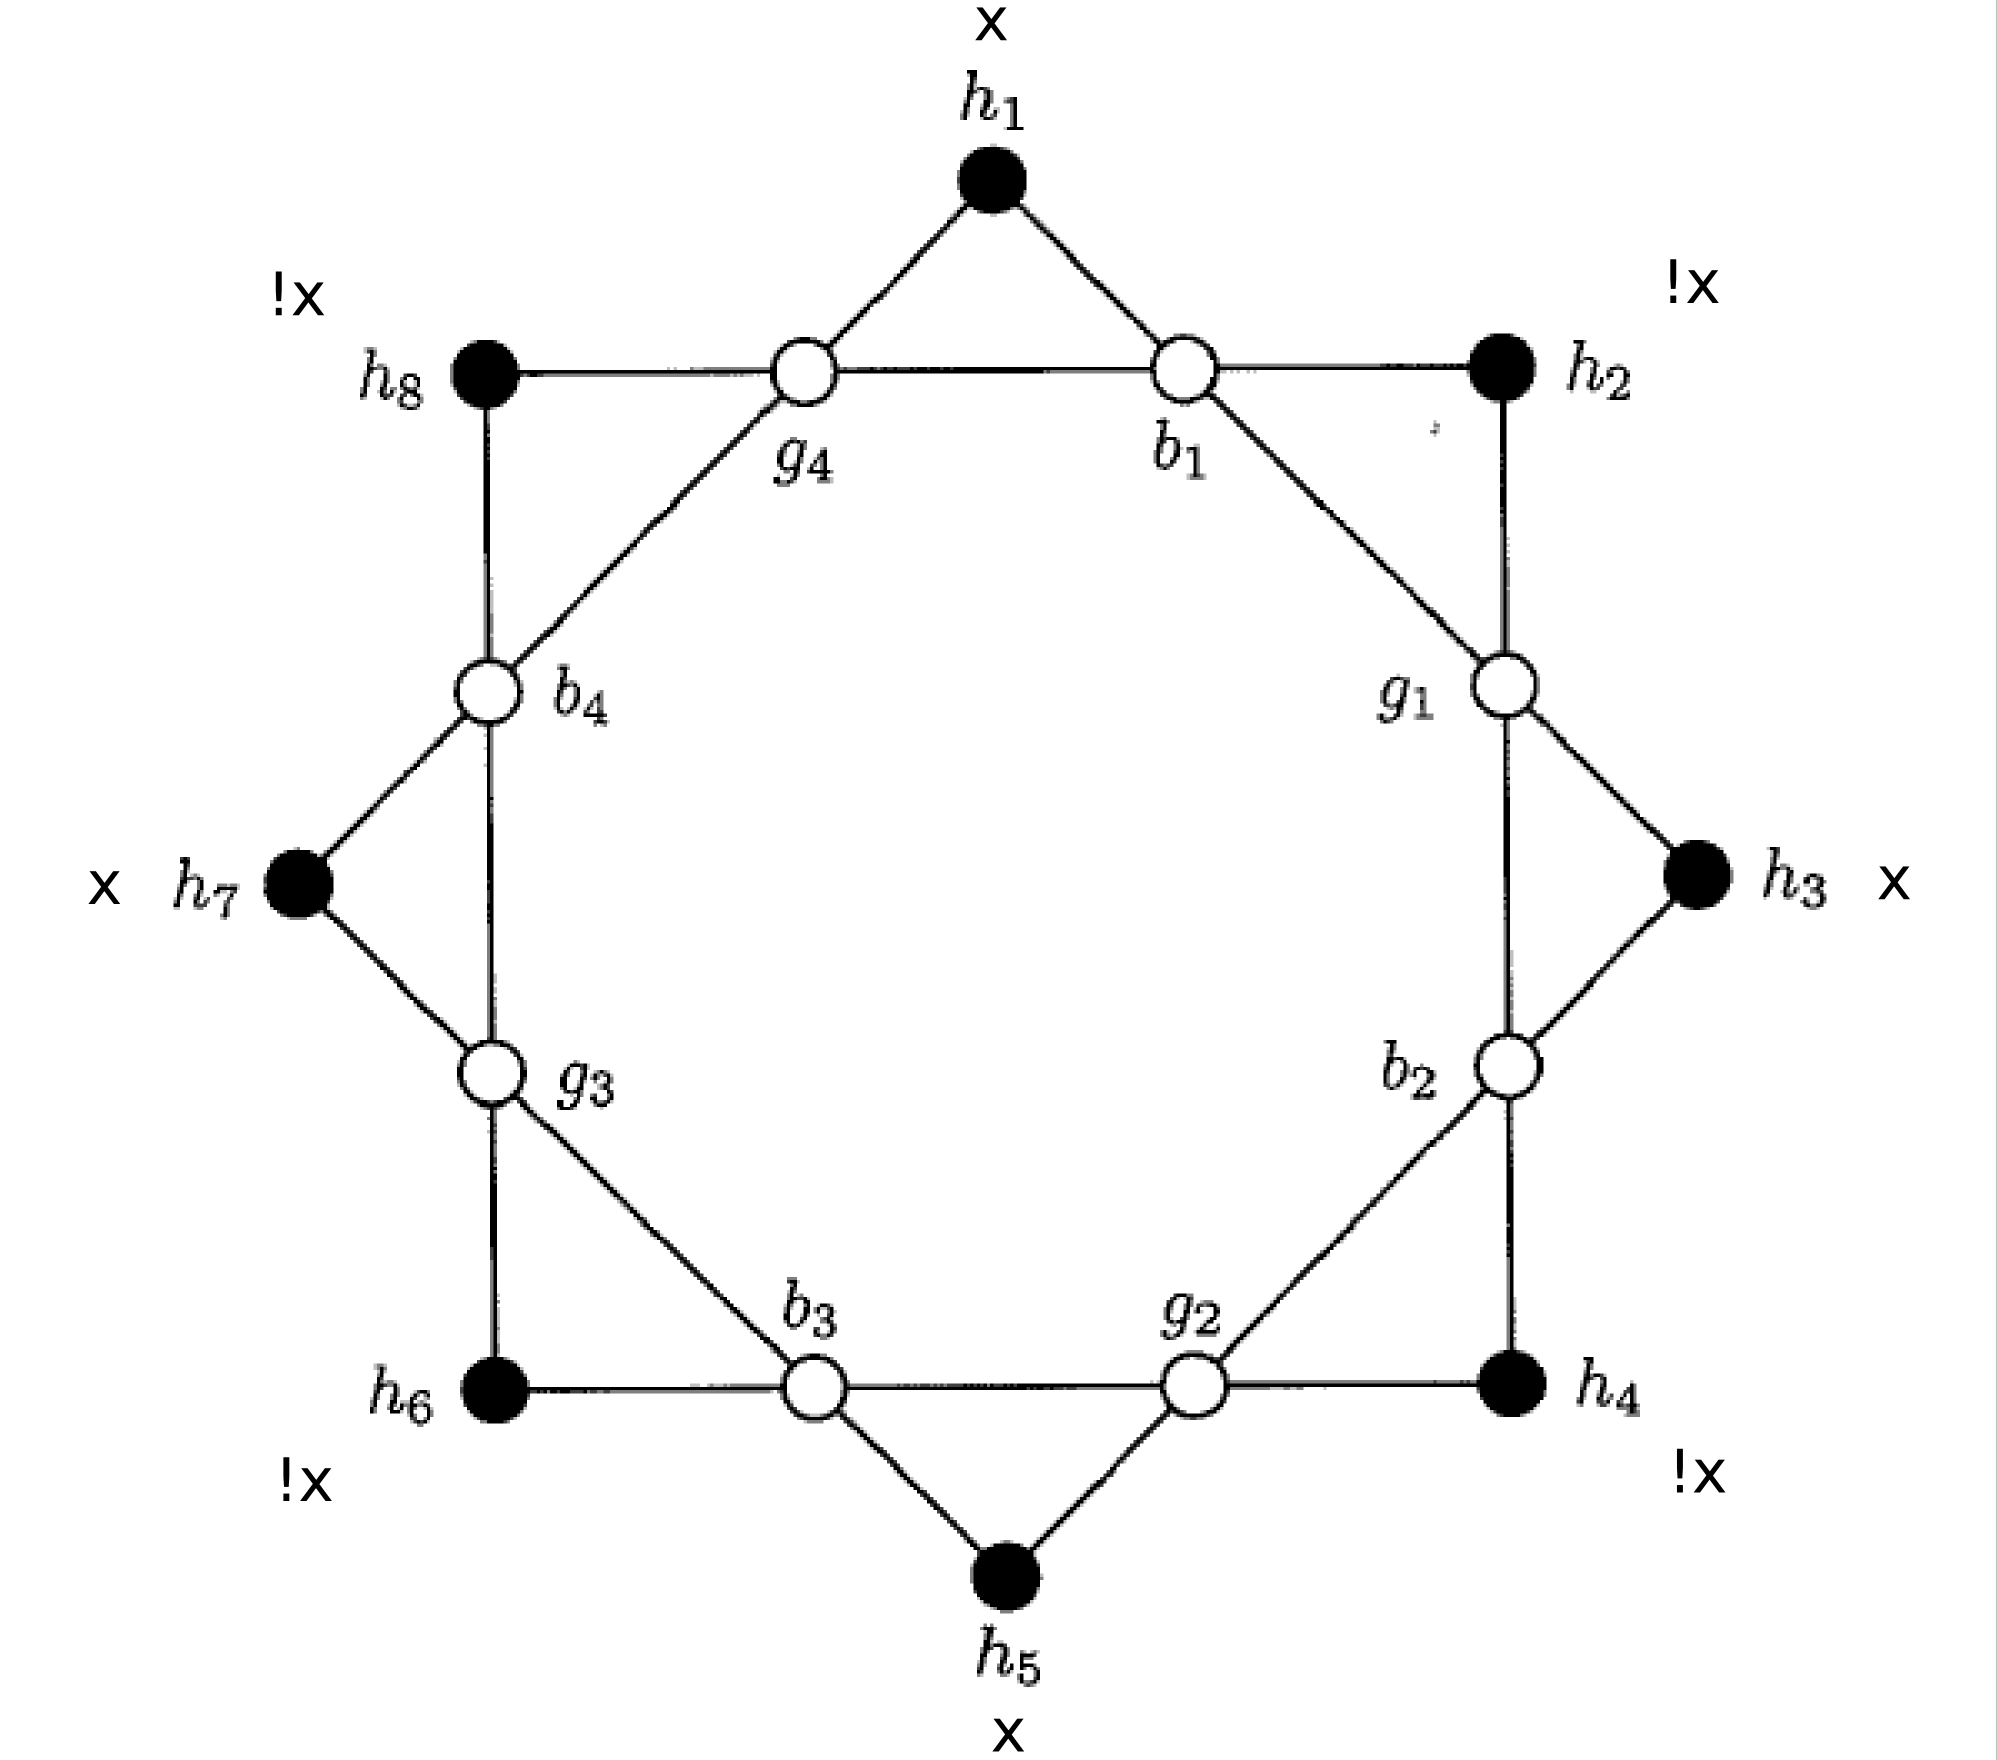
\includegraphics[bb=0 0 479 422,scale=0.5]{./choiceConsistency.png}
 % choiceConsistency.png: 1997x1760 pixel, 300dpi, 16.91x14.90 cm, bb=0 0 479 422
\end{center}
Konstruktionen følger så denne opskrift:
\begin{enumerate}
 \item For hver variabel $x_i$ i $f$, konstruer en ``choice-consistency'' gadget
    \subitem (a) Lad $k$ være antallet af forekomster af $x_i$, eller $\neg x_i$, i $f$ (den af dem hvor der er flest).
    \subitem (b) Konstruer vores gadget med $k$ drenge, $k$ piger og $2k$ hjem. Hvor drenge og piger placeres efter hinanden i en slags ``ring'' hvor hjemene er placeret ud for dem i en trekant repræsenterende tripler.
    \subitem (c) Hjemene $h_{2i-1}$ repræsenterer forekomster af $x$, hvor $h_{2i}$ repræsenterer forekomster af $\neg x$, for $i = 1,\hdots,k$. (hvis antallet af forekomster af de to er ulige, så vil nogle $h_i$'er blot være utildelt)
    \subitem (d) De $k$ drenge og $k$ piger indgår ikke i tripler af $T$ udover dem der er vist i figuren. Så hvis en matching eksisterer, så er $b_i$ matched med $g_i$ og $h_{2i}$ eller med $g_{i-1}$ ($g_k$ hvis $i=1$) og $h_{2i-1}$, for $i = 1,\hdots,k$. Hvis den første var tilfældet, så er $T(x)=true$ og hvis det er den anden så er $T(x)=false$. \\
    Dette betyder, at en given variabel $x$ altid vælger en tildeling og alle forekomster af variablen har konsistente værdier.
 \item For hver klausul i $f$, konstruer en triple med en dreng $b$ og en pige $g$. De eneste tripler $b$ og $g$ indgår i, er så tripler på formen $(b,g,h)$ hvor $h$ er de 3 hjem svarende til de 3 forekomster af literals i den pågældende klausul. Ideen er så, at hvis en af disse 3 hjem blev efterladt ubeboet når variabler blev tildelt værdier, så betyder det at huset svarer til en ``true'' literal og klausulen er derfor tilfredsstillet. Hvis alle 3 literals i klausulen er ``false'', så kan $b$ og $g$ ikke tildeles et hjem. \\
 Illustreret nedenfor:
\end{enumerate}
\begin{center}
 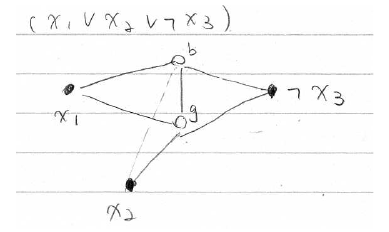
\includegraphics[bb=0 0 292 174]{./choiceConsistencySub.png}
 % choiceConsistencySub.png: 389x232 pixel, 96dpi, 10.29x6.14 cm, bb=0 0 292 174
\end{center}


Hermed er konstruktionen færdig, dog med den detalje at der pt. er flere hjem end drenge og piger i konstruktionen. Hvis der er $m$ klausuler, så er der $3m$ forekomster hvorfor der mindst er $H=3m$ hjem (for hver variabel har vi mindst lige så mange hjem som forekomster). På den anden side har vi $\frac{H}{2}$ drenge i vores gadgets og yderligere $m \leq \frac{H}{3}$ i vores klausul constraint del.

Lad os antage at mængden af huse vi har for meget er $l$, så kan vi introducere $l$ flere drenge og $l$ flere piger, således $|B| = |G| = |H|$. For hver af disse $l$ drenge og piger tilføjes så $|H|$ tripler der forbinder til alle hjem. Disse sidste $l$ drenge og piger kan så ses som ``easy to please'' par, da de blot bruges til at udfylde hvad end hjem der er ubeboet.\\
~\\
Vi påstår så nu, at en tripartite matching eksisterer hvis og kun hvis den oprindelige boolske formel var tilfredsstillet. Dette kan vi se ved 
 
\end{proof}



\subsubsection{Collary: Andre problemer med sæt i NPC}

Nu hvor vi har bevist at TRIPARTITE MATCHING er NP-Complete, så bringer det nærmest automatisk en række andre problemer ind i den kategori, da visse andre problemer med sæt blot er forskellige afarter heraf. Her kigger vi specifikt på 3 hurtigt, nemlig EXACT COVER BY 3-SETS, SET COVERING og SET PACKING. Problemerne er defineret således:

\begin{description}
 \item[SET COVERING:] Vi er givet en familie $F = \left\lbrace S_1,\hdots,S_n \right\rbrace$ af subsets af et endeligt sæt $U$ og et budget $B$. Er der et sæt af $B$ sæt i $F$ hvor deres foreningsmængde er $U$?
 \item[SET PACKING:] Vi er givet en familie $F = \left\lbrace S_1,\hdots,S_n \right\rbrace$ af subsets af et sæt $U$ og et mål $K$. Er der $K$ parvis disjunkte sæt i familien $F$?
 \item[EXACT COVER BY 3-SETS:] Vi er givet en familie $F = \left\lbrace S_1,\hdots,S_n \right\rbrace$ af subsets af et sæt $U$, således at $|U|=3m$ for en given int $m$ og $|S_i|=3$ for alle $i$. Er der $m$ sæt i $F$ som er disjunkte og har $U$ som deres foreningsmængde?
\end{description}

Alle disse problemer kan vises at være NP-Complete, da de alle er generaliseringer af TRIPARTITE MATCHING.\\
~\\
\textbf{Collary:} EXACT COVER BY 3-SETS, SET COVERING og SET PACKING $\in$ NPC

\begin{proof}
 Vi starter med at reducere TRIPARTITE MATCHING til EXACT COVER BY 3-SETS, for derved at vise, at sidstnævnte er i NPC.

 Givet sæt $B$, $G$ og $H$, samt relationen $T \subseteq B \times G \times H$ i TRIPARTITE MATCHING, så vil vi konstruere disse dele i EXACT COVER BY 3-SETS vha. en polynomiel reduktion $r$. Således kan vi sige, at EXACT COVER BY 3-SETS har $m$ sæt der er disjunkte og har foreningsmængde $U$, hvis og kun hvis TRIPARTITE MATCHING har en fyldestgørende matching.

 Måden vi gør det på er ved at dele $U$ i sidstnævnte op, således $U = B \bigcup G \bigcup H$ hvor disse $B$, $G$ og $H$ selvfølgelig er disjunkte. Til enhver triple $t_i=(b,g,h) \in T$ associerer vi så et sæt $S_i=\left\lbrace b,g,h \right\rbrace$
 Således får vi, at foreningsmængden af de $m$ sæt kun er $U$ såfremt $T$ er en fyldestgørende matching, og vice-versa.
 
 Altså har vi at EXACT COVER BY 3-SETS $\in$ NPC.\\
~\\
Et endnu nemmere bevis kan føres for SET COVERING ved at reducere fra EXACT COVER BY 3-SETS. Vi lader blot $F$ udelukkende bestå af sæts med 3 elementer, lader $U$ bestå af $3m$ elementer og sætter budgettet $B=m$, derved får vi EXACT COVER BY 3-SETS direkte. 

Så SET COVERING $\in$ NPC.\\
~\\
Det tilsvarende kan gøres igen for en reducering fra EXACT COVER BY 3-SETS til SET PACKING, hvor $F$ og $U$ sættes som før, og målet $K=m$. 

Således får vi også her at SET PACKING $\in$ NPC.
\end{proof}

\subsubsection{Theorem: (EXACT COVER BY 3-SETS $\leq$ KNAPSACK)}

Nu hvor vi har vist at EXACT COVER BY 3-SETS er NP-Complete, så kan vi nu bruge den viden til at lave endnu en reduktion. Vi vil kigge på problemet kaldet KNAPSACK.

Problemet går ud på at vi må vælge nogle genstande blandt $n$ samlede genstande. Genstand $i$ har værdi $v_i$ og vægt $w_i$, hvor begge er positive heltal. Der er desuden en max vægt på $W$, som er den maksimale vægt vores genstande tilsammen må veje. Vi skal så nu vælge genstande, uden gentagelser, således vi maksimerer den totale værdi med den constraint at den samlede vægt ikke må overstige $W$.

Vi leder altså efter et subset $S \subseteq \left\lbrace 1,\hdots,n \right\rbrace$ således at $\sum_{i \in S} w_i \leq W$ og $\sum_{i \in S} v_i$ er så stor som mulig.

I beslutningsproblem varianten har vi desuden et mål $K$ og vi ønsker at finde et subset $S \subseteq \left\lbrace 1, \hdots, n \right\rbrace$ således $\sum_{i \in S} w_i \leq W$ og $\sum_{i \in S} v_i \geq K$.

Vi vil så nu bevise at KNAPSACK $\in$ NPC ved at bevise et relateret problem.\\
~\\
\textbf{Theorem 9.10:} KNAPSACK $\in$ NPC

\begin{proof}
 I dette bevis vil vi reducere fra EXACT COVER BY 3-SETS, men vi vil ikke reducere til KNAPSACK. I stedet vil vi begrænse problemet og fokusere på et special case, som vi så vil bevise er NPC. Dette special case kalder vi SUBSET SUM og det eneste vi ændrer imellem de to, er at $K=W$ og for hver genstand $i$ sætter vi $v_i = w_i$.

Altså har vi nu et problem hvor vi er givet et sæt af $n$ heltal $v_1,\hdots,v_n$ og endnu et heltal $K$. Vi ønsker nu at finde ud af om et givet subset summer præcist op til $K$.\\

 Vi har altså en instance af EXACT COVER BY 3-SETS med sæt $\left\lbrace S_1, S_2,\hdots,S_n \right\rbrace$, hvor vi spørger om der er disjunkte sæt hvor deres foreningsmængde er sættet $U = \left\lbrace 1, 2, \hdots, 3m \right\rbrace$. Vi tænker på disse sæt som bit vektorer i $\left\lbrace 0,1 \right\rbrace^{3m}$, således de også kan tænkes som binære heltal og forening mellem disse sæt nu ligner heltalsaddition til forveksling (eksempel ses nedenfor)
\begin{center}
 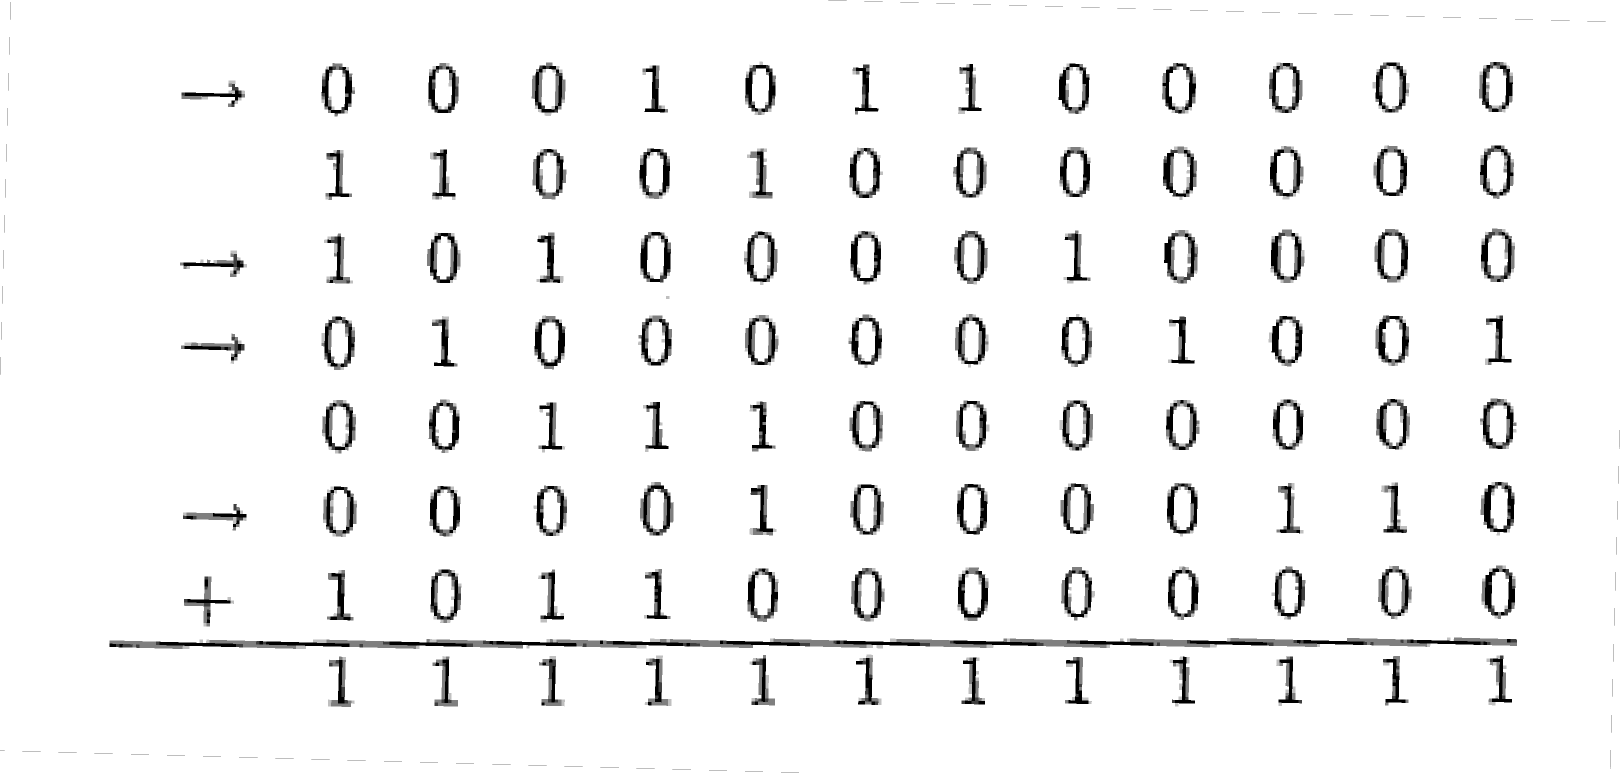
\includegraphics[bb=0 0 389 186,scale=0.5]{./KNAPSACK.png}
 % KNAPSACK.png: 1620x773 pixel, 300dpi, 13.72x6.54 cm, bb=0 0 389 186
\end{center}
Vores mål er nu at finde et subset af disse binære heltal der summerer op til $K=2^n -1$, altså en bitstreng med rene 1-taller, svarende til hele $U$. Reduktionen er nu fuldendt, men der er en mindre additionsbug. 

Problemet er, at binær heltalsaddition ikke er det samme som mængdeforening, da binær heltalsaddition har såkaldt ``carry'' (i.e. $1 + 1 \rightarrow 0, carry 1$, så $1 + 1 = 0 + 1 \times 10$ hvilket giver $10$ i binær). F.eks. er $3+5+7=15$ i bitvektorform $0011 + 0101 + 0111 = 1111$, men i de tilsvarende sæt er det $\left\lbrace 3,4 \right\rbrace, \left\lbrace 2,4 \right\rbrace$ og $\left\lbrace 2,3,4 \right\rbrace$, som er ikke disjunkte (som de burde) og deres foreningsmængde heller ikke $\left\lbrace 1,2,3,4 \right\rbrace$.

Der er dog en simpel og smart måde at undgå dette problem på. I stedet for at have disse vektorer af heltal i base 2, så hav dem i base $n+1$. På den måde bliver sæt $S_i$ til heltal $v_i = \sum_{j \in S_i} (n+1)^{3m-j}$.

Siden der nu ikke er noget ``carry'' i additionen af op til $n$ af disse numre, så er det nu klart at se, at disse heltal summer op til $K = \sum_{j=0}^{3m-1} (n+1)^j$ hvis og kun hvis der er et exact cover iblandt $\left\lbrace S_1, S_2, \hdots, S_n \right\rbrace$.

Vi har altså at EXACT COVER BY 3-SETS $\leq$ SUBSET SUM og derved at SUBSET SUM $\in$ NPC, hvilket også vil sige KNAPSACK $\in$ NPC. 
\end{proof}

